% !TeX spellcheck = el_GR-en_US
  \documentclass[11pt]{article}
  \usepackage{geometry}
  \geometry{a4paper, top=2.5cm, bottom=2.5cm, left=2.2cm,
    right=2.2cm}
  \usepackage{fontspec}
  \usepackage{titlesec}
  \usepackage{titling}
  \usepackage{float}
  \usepackage{subcaption}
  \usepackage[nonumeralsign]{xgreek}
  \usepackage{fancyhdr}
  \usepackage{hyperref}
  \usepackage{enumitem}
  \usepackage{cite}
  \usepackage{multirow}
  \usepackage{graphicx}
  \usepackage[normalem]{ulem}
  \usepackage{float}
  \restylefloat{table}
  \useunder{\uline}{\ul}{}
  \usepackage{amsmath}

  \setmainfont{Lato}
  \setmonofont{Consolas}

  \title{Τεχνολογία Ήχου και Εικόνας 2018\\
    Εργασία 2018-2019}
  \author{Χριστίνα Θεοδωρίδου - 8055\\
    Φρανκ Μπλάννινγκ - 6698\\
    Αποστόλης Φανάκης - 8261}
  \date{\today}

  \pagestyle{fancy}
  \lhead{Τεχνολογία Ήχου και Εικόνας 2018}
  \rhead{~σ}
  \renewcommand{\headrulewidth}{0.4pt}
  \renewcommand{\footrulewidth}{0.4pt}
  \setlength{\headheight}{14pt}

  \hypersetup{colorlinks=true, linkcolor=black, urlcolor=blue, citecolor=blue}
  \urlstyle{same}

  \begin{document}

  \maketitle
  \tableofcontents

  \newpage
  
  \section{Εισαγωγή}

Το ζητούμενο της εργασίας είναι η ανάπτυξη ενός μοντέλου μηχανικής
μάθησης το οποίο, παρέχοντας ένα αρχείο ήχου, θα μπορεί να ξεχωρίσει
ανάμεσα στα κομμάτια του χρόνου που περιέχουν ομιλία (speech) και
μουσική (music), όπως παρουσιάζεται στον διαγωνισμό MIREX 2018:Music and/or Speech Detection 
\footnote{https://www.music-ir.org/mirex/wiki/2018:Music\_and/or\_Speech\_Detection} .
Η εργασία επικεντρώνεται στην εύρεση των δειγμάτων που περιέχουν είτε φωνή είτε μουσική
και στην ταξινόμησή τους.

Πρόκειται για ένα δυαδικό πρόβλημα ταξινόμησης που είναι σημαντικό καθώς έχει
εφαρμογές σε πλατφόρμες κοινωνικών δικτύων για την αναγνώριση
περιεχομένου με πνευματικά δικαιώματά, σε συστήματα αυτόματης
αναγνώρισης διαφημίσεων, μοντέρνα "έξυπνα" βοηθητικά ακοής κ.α. Η
πρόσφατη βιβλιογραφία περιέχει θεματολογία όπου στοχεύει είτε στην
ανάπτυξή αλγορίθμων για γρήγορη και φθηνή υπολογιστικά ταξινόμηση,
είτε στην αναγνώριση πολύ μεγάλης ακρίβειας. Αυτό διότι αυτή τη
στιγμή η αναγνώριση με ποσοστό επιτυχίας γύρω στο 98\% είναι κάτι
συνηθισμένο.
  \section{Προηγούμενες υλοποιήσεις}

Υπάρχει πληθώρα βιβλιογραφίας σχετική με το θέμα. Έχουν βρεθεί ήδη
αρκετές λύσεις, ενώ οι πιο πρόσφατες πετυχαίνουν αξιοσημείωτα
αποτελέσματα τόσο όσων αφορά την ταχύτητα του διαχωρισμού όσο και την ακρίβεια
των αποτελεσμάτων. Κάποιες από τις δημοσιεύσεις οι οποίες αφορούν το
συγκεκριμένο θέμα, καθώς και τα αποτελέσματά τους παρουσιάζονται παρακάτω.

\vspace{1em}
Στο ~\cite{robust} οι συγγραφείς χρησιμοποιούν τα εξής χαρακτηριστικά (features):
\begin{enumerate}[noitemsep]
\item Διαμόρφωση ενέργειας στα 4Hz του σήματος (4Hz modulation)
\item Διαμόρφωση εντροπίας του σήματος (entropy modulation)
\item Αριθμός των στατικών τμημάτων
\item Διάρκεια των τμημάτων
\end{enumerate}

Παρατηρήθηκε πειραματικά ότι τα πρώτα 3 χαρακτηριστικά δίνουν ξεχωριστά περίπου
το ίδιο ποσοστό επιτυχών ταξινομήσεων (περίπου 84\%) ενώ η Μπαγιεσιανή προσέγγιση
για το χαρακτηριστικό δίαρκειας τμημάτων έδωσε λίγο χαμηλότερο ποσοστό (76.1\%). 

Για να αυξηθεί το ποσοστό των συνολικών επιτυχών ταξινομήσεων προτάθηκε ένας
ιεραρχικός αλγόριθμος ταξινόμησης στον οποίο τα χαρακτηριστικά διαμόρφωσης
ενέργειας του σήματος στα 4Ηz και διαμόρφωσης εντροπίας του σήματος συγχωνεύονται.
Σε περίπτωση που οι 2 ταξινομητές συμφωνούν αποφασίζουν για το αν το τμήμα
αποτελεί ομιλία ή όχι, ενώ σε περίπτωση που δεν συμφωνούν, η απόφαση
οριστικοποιείται από το χαρακτηριστικό του αριθμού τμημάτων. Αποδεικνύεται ότι
τα αποτελέσματα αυτού του αλγορίθμου δίνουν 90.1\% σωστές ταξινομήσεις.

\vspace{1em}
Στο ~\cite{mirex} το πρόβλημα που δόθηκε αντιμετωπίζεται ως 2 υποπροβλήματα:
το πρόβλημα εντοπισμού δειγμάτων και το πρόβλημα κατηγοριοποίησής τους.
Για τον εντοπισμό δειγμάτων μουσικής/φωνής εφαρμόστηκε ο αλγόριθμος Random
Forest σε 2 εκδοχές του: στην πρώτη, εφαρμόστηκε μαζί με έναν Silence detection
αλγόριθμο ενώ στη δεύτερη βασίστηκε μόνο στις πληροφορίες ομοιογένειας (self
similarity matrix) και στην λειτουργία του ίδιου του ταξινομητή. Επίσης, για την
ταξινόμηση προτάθηκαν 2 εναλλακτικές: στην πρώτη χρησιμοποιήθηκε ένα
προ-εκπαιδευμένο μοντέλο ενώ στην δεύτερη η εκπαίδευση γίνεται κατά την
αξιολόγηση των δειγμάτων.

Χρησιμοποιήθηκαν τα χαρακτηριστικά (features):
\begin{enumerate}[noitemsep]
\item RMS ενέργεια
\item ZCR (Zero-Crossing Rate)
\item Spectral rolloff (Συχνότητα Αποκοπής)
\item Spectral flux (Φασματική Ροή)
\item Spectral flatness (Φασματική Επιπεδότητα)
\item Spectral flatness per Band (Φασματική Επιπεδότητα ανά συχνοτικές ομάδες)
\item MFCCs (Mel Frequency Cepstral Coefficients)
\end{enumerate}

% TODO: η παράγραφος δε βγάζει και πολύ νόημα μετά από ένα σημείο
Έγινε ανάλυση κύριων συνιστωσών (Principal component analysis ή PCA) με στόχο να
μειωθούν οι διαστάσεις των διανυσμάτων των χαρακτηριστικών (feature vectors).
Δημιουργήθηκαν οι πίνακες ομοιότητας υπολογίζοντας την ευκλείδεια απόσταση
μεταξύ των δειγμάτων ήχου έτσι ώστε να χωριστούν σε τμήματα. Στη συνέχεια τα
τμήματα αυτά κατηγοριοποιούνται ενώ ταυτόχρονα εφαρμόζεται ο αλγόριθμος Silence
Detection. Για το πρόβλημα της
κατηγοριοποίησης χρησιμοποιείται ο ίδιος αλγόριθμος Random Forest για
ταξινόμηση σε επίπεδο τμημάτων ήχου (frame). Εφόσον για κάθε αρχείο ήχου έχουν
εξαχθεί τα παραπάνω χαρακτηριστικά, κάθε τμήμα ήχου ταξινομείται στην κλάση που
αποφασίζεται και έπειτα ολόκληρο το αρχείο ταξινομείται στην κλάση στην οποία
ταξινομήθηκαν τα περισσότερα τμήματά του.

\vspace{1em}
Στο ~\cite{speech} προτείνεται πως τα χαρακτηριστικά μπορεί να μην καλύπτουν
χαρακτηριστικά και της ομιλίας και της μουσικής, αλλά να βασίζονται κυρίως σε
χαρακτηριστικά ενός από τα δύο. Ενδιαφέρον παρουσιάζουν τα χαρακτηριστικά της
ομιλίας, τα οποία λόγω των μέσων που την παράγουν (τα χείλη, η γλώσσα και οι
φωνητικές χορδές) έχουν ιδιαίτερα γνωρίσματα. Η μελέτη αυτών των χαρακτηριστικών
και η χρήση τους σε έναν ταξινομητή αποδεικνύεται πως μπορεί να
αυξήσει την επιτυχία του διαχωρισμού.

Ενδεικτικά, πέρα από το καθιερωμένο χαρακτηριστικό της διαμόρφωσης ενέργειας στα 4Hz (4Hz modulation energy), λόγω του
ρυθμού των συλλαβών, κάποια άλλα χαρακτηριστικά ειδικά για ομιλία βασίζονται στην
αναγνώριση του ήχου που παράγεται στις φωνητικές χορδές κατά την εναλλαγή της
προφοράς ενός συμφώνου σε ένα φωνήεν ή στην μελέτη της αυτοσυσχέτησης του
σήματος μετά από φιλτράρισμα (Zero Frequency Filtered Signal).

\vspace{1em}
Πέρα από την επιλογή των χαρακτηριστικών, η μέθοδος εκπαίδευσης έχει μεγάλη επίπτωση στην
τελική αποτελεσματικότητα του αλγορίθμου. Μερικές φορές χρήση σύνθετων μεθόδων
εκπαίδευσης μπορούν να επιφέρουν καλύτερα αποτελέσματα σε μεγαλύτερο ποσοστό
διότι επιτρέπουν την έξοδο από τοπικά ελάχιστα. Η σύνθετες μέθοδοι μπορεί να μην
είναι συμβατικές ή και να δανείζονται από παρατηρήσεις της φύσης, όπως ο
συνδυασμός ενός Support Vector Machine (SVM) με τον Cuckoo Algorithm ~\cite{cuckoo},
όπου, όπως το πουλί κούκος που γεννάει τα αυγά του σε ξένες φωλιές, στις
επαναλήψεις εκπαίδευσης του SVM κάποιες λύσεις πετιούνται και αντικαθίστανται από
νέες οι οποίες μπορεί να επιφέρουν καλύτερα αποτελέσματα.

\vspace{1em}
Στο ~\cite{hybrid} οι συγγραφείς χρησιμοποιούν τα χαρακτηριστικά:
\begin{enumerate}[noitemsep]
\item ΜFCCs (Mel Frequency Cepstral Coefficients)
\item ZCR (Zero-Crossing Rate)
\item SC (Spectral Centroid)
\item SR (Spectral Rolloff)
\item SF (Specral Flux)
\end{enumerate}

Τα χαρακτηριστικά ΜFCC, ZCR και SF ταξινομούν με ακρίβεια ~90\% το καθένα. Το SR με 83\%, ενώ το SC με 70\%. Ο συνδυασμός όλων των παραπάνω χαρακτηριστικών πετυχαίνει
93.5\% σωστή ταξινόμηση, ενώ με χρήση ενός SVM μοντέλου το ποσοστό φτάνει στο
95.68\%.

Παρατηρείται ότι η σωστή ταξινόμηση της μουσικής είναι αρκετά δυσκολότερη (με
τα συγκεκριμένα χαρακτηριστικά) σε σχέση με αυτή της ομιλίας. Ειδικότερα στην ομιλία
επιτυγχάνεται (με το SVM) ακρίβεια 98.25\% ενώ στη μουσική 93.1\%.

\vspace{1em}
Τέλος, σύμφωνα με το ~\cite{radio}, σε εφαρμογές κατηγοριοποίησης όπου δεν
επιβάλλεται η λειτουργία σε πραγματικό χρόνο, η χρήση χαρακτηριστικών ενέργειας είναι
επιθυμητή λόγω της μεγάλης ακρίβειας τους. Συγκεκριμένα η αναζήτηση της ελάχιστης πυκνότητας ενέργειας (Minimum
Energy Density) δείχνει να υπερέχει από άλλα χαρακτηριστικά ενέργειας τόσο στην
αποτελεσματικότητα της όσο και στην απλότητα του υπολογισμού της. Σε συνδυασμό με το
χαρακτηριστικό της διαφοράς ενέργειάς στα διάφορα κανάλια μιας πολυκάναλης
εισόδου, στο ~\cite{radio} πέτυχαν ακρίβεια 100\% στα κομμάτια εισόδου όπου
περιείχαν μόνο μουσική ή ομιλία και όχι τον συνδυασμό τους (όπως στις ραδιοφωνικές
διατιμήσεις).

  % \section{Σχεδιασμός υλοποίησης}

Μετά από μελέτη των προηγούμενων υλοποιήσεων και πειραματισμό με την εξαγωγή
διάφορων χαρακτηριστικών (features) στη Matlab αποφασίσαμε να ακολουθήσουμε την
παρακάτω πορεία αντιμετώπισης του προβλήματος.

\subsection{Παραθυροποίηση}

Για την παραθυροποίηση του σήματος θα γίνει χρήση Hamming παραθύρων με επικάλυψη
50\%. Η τελική χρονική διάρκεια των παραθύρων αναμένεται να είναι στο πεδίο του
μισού με ενός δευτερολέπτου (0.5-1 sec) και θα καθοριστεί στη πορεία μέσω trial
and error τεχνικών.

\subsection{Χαρακτηριστικά}

Τα χαρακτηριστικά που έχουν επιλεγεί είναι τα εξής:
\begin{enumerate}[noitemsep]
\item ΜFCCs (Mel Frequency Cepstral Coefficients)
\item Silence ratio
\item ZCR (Zero-Crossing Rate)
\item SC (Spectral Centroid)
\item SR (Spectral Rolloff)
\item SF (Specral Flux)
\item 4Hz modulation
\item Minimum Energy Density (MED)
\end{enumerate}

Τα συγκεκριμένα χαρακτηριστικά εμφανίζουν τις μεγαλύτερες ακρίβειες στη
ταξινόμηση ενώ ταυτόχρονα έχουν μικρή ετεροσυσχέτιση. Άλλα χαρακτηριστικά μπορεί
να προστεθούν στη πορεία μετά από αναλυτικότερη έρευνα της βιβλιογραφίας.

\subsection{Μοντέλο ταξινόμησης}

Από την βιβλιογραφική έρευνα διαπιστώθηκε ότι οι διαφορετικές επιλογές
χαρακτηριστικών επηρεάζουν την ακρίβεια των μοντέλων. Έτσι με μία συγκεκριμένη
επιλογή χαρακτηριστικών μπορεί τα πιθανοτικά μοντέλα (Naive Bayes, GMM, κ.α.) να
είναι αποτελεσματικότερα των SVM ή των νευρωνικών. Αλλά με επιλογή διαφορετικών
features να ισχύει το αντίθετο. Για τον λόγο αυτό είναι απαραίτητο, αφού
αποφασιστεί το σετ των χαρακτηριστικών να γίνει εκπαίδευση και testing πολλών
μοντέλων πριν την τελική επιλογή.
Έτσι η πρόταση μας είναι η δοκιμή των περισσότερων ευραίως διαδεδομένων μοντέλων,
όπως: Decision trees, Bayesian networks, Gaussian mixture model, Hidden Markov
Model, SVMs, Artificial Neural networks, Genetic Algorithms.

\subsection{Preprocessing, άλλες τεχνικές}

Περισσότερες και πιο εξεζητημένες τεχνικές θα χρησιμοποιηθούν στο πρακτικό
κομμάτι που θα υλοποιηθεί αργότερα. Κατά το preprocessing των δεδομένων μέθοδοι
όπως data rescaling, data standardization, data binarization, data cleaning,
data integration, data transformation ενδέχεται να φανούν χρήσιμες. Ακόμα, κατά
την εκπαίδευση διάφορες γνωστοί μέθοδοι validation όπως το k-fold cross-validation,
leave one out, bootstrap, hold out θα δοκιμαστούν.

\subsection{Stack}

Τόσο για την εξερεύνηση του χώρου των χαρακτηριστικών όσο και για την εκπαίδευση
και τον έλεγχο του μοντέλου θα χρησιμοποιηθεί το προγραμματιστικό περιβάλλον της
R. Το περιβάλλον αυτό είναι ειδικά σχεδιασμένο για στατιστικούς υπολογισμούς
(statistical computing) και αποτελεί (μαζί με την python) το στάνταρ της
βιομηχανίας μηχανικής μάθησης. Επίσης παρέχεται αφθονία βιβλιοθηκών έτοιμων
machine learning αλγορίθμων από τις οποίες θα χρησιμοποιηθούν μεταξύ άλλων οι:
'e1071', 'rpart', 'nnet', 'random forest'.

Σε διάφορα στάδια της εργασίας ενδέχεται να χρησιμοποιηθεί και η γλώσσα Matlab
λόγω της ευκολίας που προσφέρει στους μαθηματικούς υπολογισμούς.

  \section{Η υλοποίησή μας}

Η υλοποίησή αναπτύχθηκε σε γλώσσα Python και χρησιμοποιήθηκαν πληθώρα βιβλιοθηκών όπως η essentia για την εξαγωγή χαρακτηριστικών, η sklearn για την προεπεξεργασία δεδομένων
ενώ στην εκπαίδευση των μοντέλων χρησιμοποιήθηκε η numpy. Χρησιμοποιήθηκε επίσης η  seaborn για την εξαγωγή διαγραμμάτων και την οπτικοποίηση των χαρακτηριστικών. Παράλληλα, σε συνδυασμό με όλες αυτές χρησιμοποιήθηκαν και άλλες βιβλιοθήκες όπως η pandas,  η matplotlib, η multiprocessing, η  οs, η pyaudio κα. Για την εκπαίδευση, δοκιμάστηκαν τα μοντέλα svm, decision trees, multilayer perceptron, Naive bayes και random forest, τα οποία θα αναπτυχθούν στα επόμενα κεφάλαια. Το dataset που χρησιμοποιήθηκε για την εκπαίδευση του μοντέλου είναι το προτινόμενο GTZAN dataset \footnote{http://opihi.cs.uvic.ca/sound/music\_speech.tar.gz}, το οποίο αποτελείται απο 120 αρχεία διάρκειας 30 δευτερολέπτων. Κάθε κλάση (μουσική/φωνή) αποτελείται από 60 αρχεία ενώ δεν υπάρχουν αρχεία που να περιέχουν και τις δύο κλάσεις. Όλα τα δείγματα είναι στα 22050 Hz, Mono 16-bit και σε αρχεία μορφής .wav. Τέλος, χρησιμοποιήθηκε 4-fold cross validation για την εκτίμηση της απόδοσης του μοντέλου.

\section{Χαρακτηριστικά και προεπεξεργασία δεδομένων}

Για την εξαγωγή των χαρακτηριστικών που φαίνονται στο από τα αρχεία ήχουν του σετ δεδομένων, αρχικά τμηματήσαμε κάθε σήμα αρχείου σε frames με μέγεθος 6144 δείγματα, το οποίο προέκυψε μετά από επαναλαμβανόμενες δοκιμές.
 Έπειτα, τα frames αυτά, παραθυροποιήθηκαν με παράθυρο τύπου Hamming, ίσου μεγέθους. Στη συνέχεια, έγινε η εξαγωγή των χαρακτηριστικών στο πεδίο του χρόνου, καθώς και στο πεδίο της συχνότητας.Παράλληλα, έγινε και η εξαγωγή των συντελεστών MFCC έτσι ώστε να είναι εφικτός ο υπολογισμός της διαμόρφωσης της ενέργειας σήματος στα 4 Ηz. Τα χαρακτηριστικά που εξήχθηκαν είναι 27 και θα αναλυθούν στη συνέχεια. Ως προεπεξεργασία, τα δεδομένα κλιμακοποιήθηκαν έτσι ώστε να έχουν μέσο 0 και τυπική απόκλιση ίση με 1 για κάθε ένα. Τέλος, δίνεται η δυνατότητα στον κώδικά να εφαρμοστεί και η μέθοδος Principal Component Analysis - PCA,αν αυτή είναι αναγκαία, έτσι ώστε να μειωθούν οι τελικές διαστάσεις των χαρακτηριστικών. Στην συγκεκριμένη υλοποίηση, μειώνονται οι διαστάσεις από 27 σε 10, έτσι ώστε η διαφορά να είναι αξιοσημείωτη και να ελεγθεί τι γίνεται σε αυτήν την περίπτωση με την απόδοση.  

%pinakas me arxikes kai telikes diastaseis xarakthristikwn
% \begin{center}
% \begin{tabular}{ |c |c| }
% \hline
%  cell1 & cell2 & cell3 \\ 
%  cell4 & cell5 & cell6 \\  
%  cell7 & cell8 & cell9    
%  \hline
% \end{tabular}
% \label{table:1}
% \end{center}

\subsection{Zero Crossing Rate - ZCR}

Είναι ο ρυθμός της αλλαγής προσήμου κατά τη διάρκεια του σήματος, δηλαδή ο ρυθμός με τον οποίο το σήμα αλλάζει από θετικό και αρνητικό και αντίστροφα. Σε κάποιο βαθμό, δείχνει την μέση συχνότητα του σήματος ως εξής:
\begin{equation}
\text{ZCR} = \frac{\sum_{m=1}^{N} |sgn ~x(n) - sgn~x(n-1)| }{2N}
\end{equation}

όπου sgn() η συνάρτηση προσήμου και x(m) το διακριτό σήμα ήχου. Στη γενική περίπτωση, το ZCR για την μουσική είναι αρκετά υψιλότερο από ότι στην φωνή.

% \begin{figure}[H]
% \begin{subfigure}{.5\textwidth}
%   \centering
%   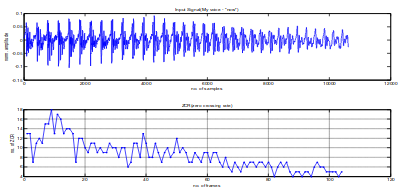
\includegraphics[width=.8\linewidth]{humanvoice.png}
%   \caption{Φωνή}
%   \label{fig:sfig1}
% \end{subfigure}%
% \begin{subfigure}{.5\textwidth}
%   \centering
%   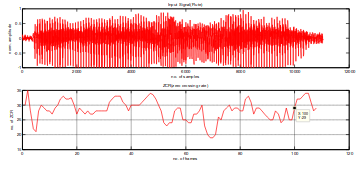
\includegraphics[width=.8\linewidth]{musicinstr.png}
%   \caption{Μουσική}
%   \label{fig:sfig2}
% \end{subfigure}
% \caption{Σήματα φωνής και μουσικής με τα αντίστοιχα ZCR \footnote{Discrimination between Speech and Music signal, Sumit Kumar Banchhor,International Journal of Soft Computing and Engineering (IJSCE)}}
% \label{fig:fig}
% \end{figure}

\subsection{Spectral Centroid - SC}

Το spectral cendroid ή αλλιώς φασματικό κέντρο, όπως αναφέρεται στο \footnote{
Speech and Music Classification and Separation: A Review 
Abdullah I. Al-Shoshan
Department of Computer Science, College of Computer, 
Qassim University, Saudi Arabia },είναι μία μετρική που χρησιμοποιείται ώστε να χαρακτηρίσει ένα φάσμα. Υποδεικνύει πού βρίσκεται το κέντρο του φάσματος. Έχει ισχυρή σύνδεση με την "φωτεινότητα " ενός ήχου δηλαδή με την χροιά. Συνήθως, το κέντρο του φάσματος της φωνής συγκεντρώνεται σε χαμηλές συχνότητες και έπειτα συμπτύσσεται πολύ γήργορα στις υψιλότερες συχνότητες ενώ δεν υπάρχει DC συνιστώσα. Αντίθετα, στην μουσική δεν έχει παρατηρηθεί κάποιο συγκεκριμένο σχήμα του φάσματος. 
\subsection{Roll Off}
 
 Το συγκικριμένο χαρακτηριστικό αναπαριστά την τιμή της συχνότητας, κάτω από την οποία βρίσκεται το 95\% της ενέργειας του σήματος. Όπως προαναφέρθηκε, η ενέργεια του μουσικού σήματος συγκεντρώνεται σε υψηλότερες συχνότητες σε σχέση με το φωνητικό σήμα. Η μαθηματική του έκφραση δίνεται ως:
 \begin{equation}
 \sum_{k<v} X(k) = 0.95 \cdot \sum_{k}X(k)
 \end{equation}
 όπου το X(k) είναι ο διακριτός μετασχηματιμός Fourier (DFT) του x(t),το αριστερό μέρος της παραπάνω εξίσωσης είναι το άθροισμα της ενέργειας κάτω από την συχνότητα v, ενώ το δεξί είναι 95\% της συνολικής ενέργειας του σήματος στο συγκεκριμένο χρονικό frame.

 \subsection{Spectral Flux}

 Το χαρακτηριστικό Spectral Flux ή αλλιώς της φασματικής ροής, όπως αναφέρεται στο 
 cite to oparapanw footnote
 μετράει την φασματική διαφορά ανάμεσα στα frames. Η μουσική έχει μεγαλύτερο ρυθμό διαφοράς ενώ έχει πιο δραστικές αλλαγές ανάμεσα στα frames από ότι η φωνή. Σημειώνεται ότι η μουσική εναλλάσσεται ανάμεσα σε περιόδους μετάβασης και στατικές περιόδους ενώ η φωνή, γενικότερα, έχει έναν πιο σταθερό ρυθμό εναλλαγών. Ως αποτέλεσμα, η τιμή της φασματικής ροής είναι υψηλότερη για την μουσική σε σχέση με την φωνή.

  \subsection{Envelope}

Το envelope είναι ουσιαστικά μία ομαλή καμπύλη που καλύπτει το περίγραμμα ενός ταλαντούμενού σήματος.Εκφράζει, ουσιαστικά, τις χρονικές αλλαγές στο πλάτο του σήματος.Οι αλλαγές αυτές είναι υπεύθυνες για πολλές πτυχές της ακουστικής αντίληψης, συμπεριλαμβανομένου της έντασης, της χροιάς, της οξύτητας και τις χωρικής ακουστότητας.


\subsection{Flatness}

To flatness ή αλλιώς επιπεδότητα του ήχου, είναι μία μετρική η οποία χρησιμοποιείται στην ανάλυση ψηφιακών σημάτων για να χαρακτηρίσει το φάσμα ενός ηχητικού σήματος. Συνήθως μετριέται σε decibels(DB), και αποτελεί έναν τρόπο να ποσοτικοποιήσει το πόσο κοντά είναι ένας ήχος σε θόρυβο και πόσο σε τονικότητα.  \footnote{https://en.wikipedia.org/wiki/Spectral\_flatness} Η αναφορά στην τονικότητα γίνεται με την έννοια του αρίθμού των κορυφών σε ένα φάσμα συχνοτήτων που θα υπήρχαν λόγω των πολλαπλών ημιτόνων σε αντίθεση με το επίπεδο φάσμα του λευκού θορύβου. Τα μουσικά σήματα, τείνουν να αποτελούνται από πολλαπλούς τόνους, ο καθένας με την δική του κατανομή αρμονικών ενώ στην φωνή δεν εμφανίζεται αυτό.


\subsection{Perceptual attack time}

Αυτό το χαρακτηριστικό αναφέρεται στην χρονική διάρκεια ανάμεσα στη χρονική στιγμή που το σήμα γίνεται ακουστικά αντιληπτό μέχρι τη χρονική στιγμή που φτάνει την μέγιστη έντασή του. 

\subsection{Sound Decay}

Η προοδευτική μείωση του πλάτους ενός σήματος με την πάροδο του χρόνου. Αυτή η φάση ξεκινάει μόλις το perceptual attack time φτάσει στο μέγιστό του. Σε αυτήν την φάση το πλάτος του σήματος μειώνεται μέχρι να φτάσει σε ένα συγκεκριμένο πλάτος στο οποίο διατηρείται μέχρι να αρχίσει να σβήνει.


\subsection{Spectral Complexity}
 
 To spectral complexity ή αλλιώς η φασματική πολυπλοκότητα, βασίζεται στον αριθμό των κορυφών του φάσματος του σήματος.

\subsection{Mel Frequency Cepstral Coefficient - MFCC }

Στην επεξεργασία ήχου, το cepstrum συχνοτήτων Mel (Μel frequency cepstrum - MFC)
είναι μια αναπαράσταση του βραχυπρόθεσμου φάσματος έντασης ενός ήχου, βασισμένου σε έναν γραμμικό μετασχηματισμό συνημιτόνου του λογαριθμισμένου φάσματος έντασης σε μια μη γραμμική κλίμακα της συχνότητας (μη γραμμικής κλίμακας Mel).  Οι συντελεστές του cepstrum συχνότητας Μελ (MFCCs – Mel Frequency Cepstrum Coefficients) είναι οι συντελεστές εκείνοι που αποτελούν στο σύνολο τους το φάσμα MFC.


\subsection{4Hz Energy Modulation}

Τα φωνητικά σήματα έχουν χαρακτηριστικό μέγιστο στη διαμόρφωση ενέργειας γύρω στα 4Hz του ρυθμού συλλαβών. Για να μοντελοποιηθεί αυτή η ιδιότητα ακολουθείται η παρακάτω διαδικασία:\footnote{https://www.irit.fr/recherches/SAMOVA/FeaturesExtraction.htm\#me4hz} Το σήμα τμηματοποιείται σε frames και εξάγονται οι Mel Frequency Spectrum Coefficients \footnote{https://en.wikipedia.org/wiki/Mel-frequency\_cepstrum} και υπολογίζεται η ενέργεια σε 40 κανάλια αντίληψης. Αυτή η ενέργεια έπειτα φιλτράρεται με ένα ζωνοδιαβατό φίλτρο, κεντραρισμένο στα 4Hz. Η ενέργεια αθροίζεται για όλα τα κανάλια, και κανονικοποιείται με βάση το μέσο του κάθε frame. Η διαμόρφωση δίνεται από τον υπολογισμό της μεταβλητότητας της φιλτραρισμένης ενέργειας σε dB σε ένα δευτερόλεπτο του σήματος. Η φωνή περιέχει περισσότερη διαμόρφωση από την μουσική.
%Leptomeries gia tin diki mas ulopoihsh, epilogh timwn ktl


\par Παρακάτω φαίνονται ενδεικτικά κάποια από τα παραπάνω χαρακτηριστικά και το πόσο αποτελεσματικά είναι στον διαχωρισμό:

\begin{figure}[H]
\centering
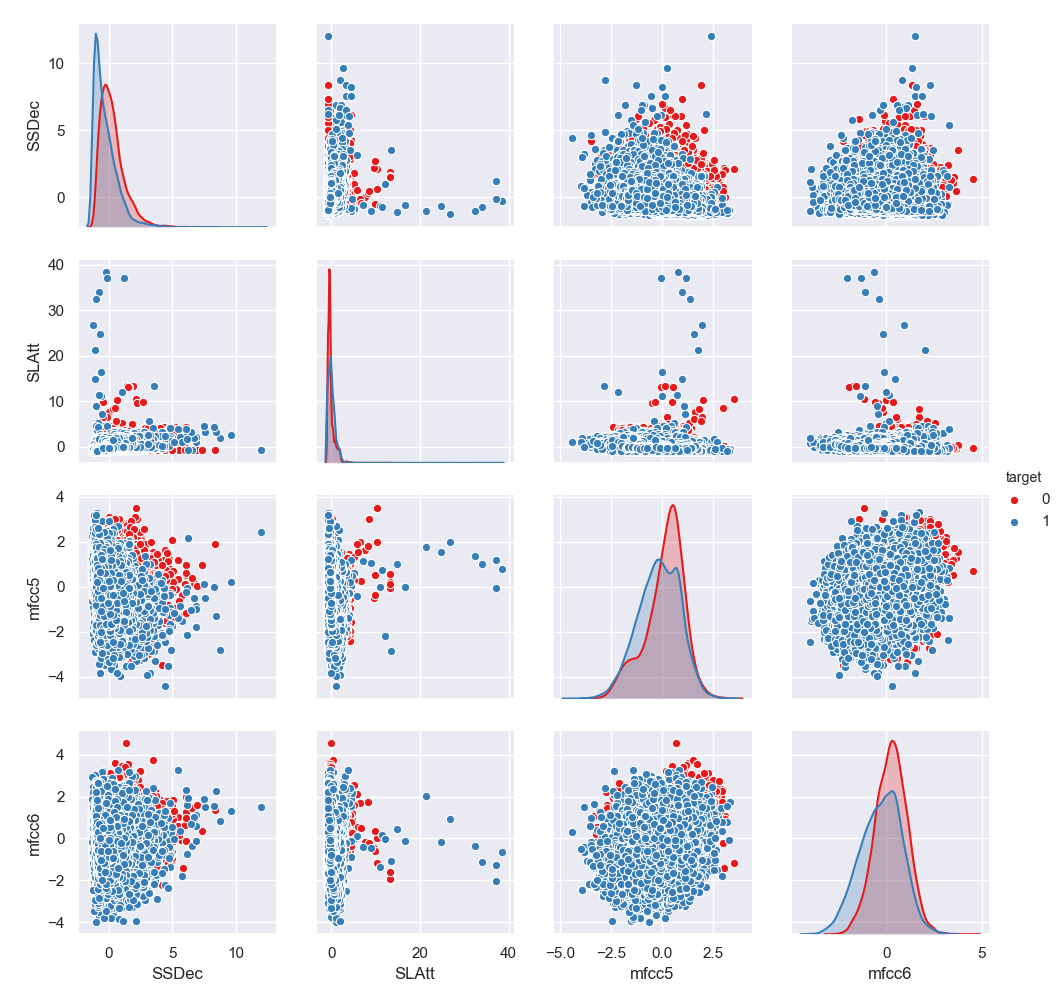
\includegraphics[width=0.7\textwidth]{figure_1.png}
\end{figure}
\begin{figure}[h]
\centering
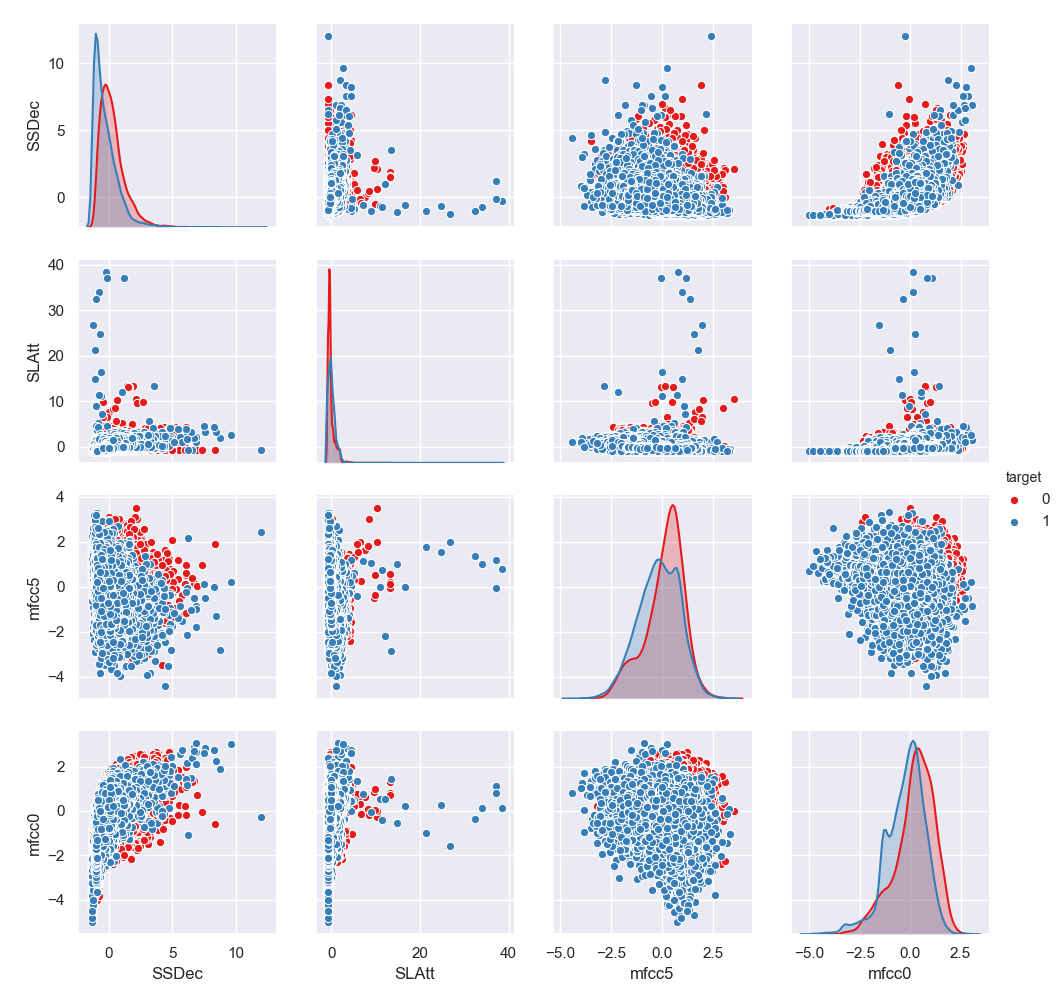
\includegraphics[width=0.7\textwidth]{figure_2.png}
\caption{Αποτελεσματικότητα χαρακτηριστικών στον διαχωρισμό των κλάσεων}
\end{figure}


Eπιπλέον, ελέγξαμε όλα τα χαρακτηριστικά ένα προς ένα έτσι ώστε να δούμε εάν υπάρχει τρόπος να φτάσουμε την πλήρη ακρίβεια του μοντέλου μας με λιγότερα ή να φτάσουμε αρκετά κοντά ίσως ακόμα και με μόνο ένα χαρακτηριστικό. 
Tα αποτελέσματα έδειξαν ότι κανένα χαρακτηριστικό από μόνο του δεν είναι ικανό να δώσει ικανοποιητικό ποσοστό ακρίβειας στο μοντέλο. Αν πάρουμε το καλύτερο σε όρους ακρίβειας και το δοκιμάσουμε σε συνδυασμό με τα επόμενα καλύτερα, φαίνεται ότι η ακρίβεια αυξάνεται λίγο αλλά όχι αρκετά.  
Τέλος, αν επαναληφθεί ακόμα μία φορά η διαδικασία, φαίνεται ότι έχουμε και πάλι μια μικρή αύξηση στην ακρίβεια, η οποία όμως είναι αρκετά μακρυά από την ακρίβεια που επιτυγχάνεται εν τέλει. 

\begin{table}[H]
\begin{tabular}{llll}
{\ul \textbf{Accuracy}} & {\ul \textbf{Individually}} & {\ul \textbf{with best 1}} & {\ul \textbf{with best 2}} \\
4Hz Mod                 & 0.58                        & 0.66                       & 0.73                       \\
Flat                    & 0.63                        & 0.71                       & 0.75                       \\
HFC                     & 0.58                        & 0.65                       & 0.72                       \\
LAtt                    & 0.62                        & 0.71                       & 0.75                       \\
SC                      & 0.59                        & 0.66                       & 0.73                       \\
Scomp                   & 0.57                        & 0.66                       & 0.73                       \\
SDec                    & 0.63                        & 0.65                       & 0.72                       \\
SEFlat                  & 0.51                        & 0.65                       & 0.72                       \\
SF                      & 0.55                        & 0.69                       & 0.75                       \\
SFlat                   & 0.57                        & 0.66                       & 0.72                       \\
SLAtt                   & 0.63                        & 0.71                       & 0.74                       \\
SR                      & 0.60                        & 0.66                       & 0.72                       \\
SSDec                   & \textbf{0.65}               & -                          & -                          \\
ZCR                     & 0.58                        & 0.65                       & 0.72                       \\
mfcc0                   & 0.61                        & 0.66                       & 0.73                       \\
mfcc1                   & 0.58                        & 0.67                       & 0.73                       \\
mfcc2                   & 0.52                        & 0.66                       & 0.73                       \\
mfcc3                   & 0.56                        & 0.69                       & 0.76                       \\
mfcc4                   & 0.54                        & 0.67                       & 0.74                       \\
mfcc5                   & 0.57                        & 0.70                       & 0.75                       \\
mfcc6                   & 0.61                        & \textbf{0.72}              & -                          \\
mfcc7                   & 0.57                        & 0.68                       & 0.75                       \\
mfcc8                   & 0.55                        & 0.67                       & 0.74                       \\
mfcc9                   & 0.54                        & 0.67                       & 0.73                       \\
mfcc10                  & 0.54                        & 0.65                       & 0.73                       \\
mfcc11                  & 0.51                        & 0.66                       & 0.73                       \\
mfcc12                  & 0.54                        & 0.67                       & 0.73                      
\end{tabular}
\caption{Ακρίβεια μεμονωμένων χαρακτηριστικών και συνδυασμών τους}
\end{table}

%Διαγραμμα features-απόδοσης;
Άρα, είναι προφανές ότι δεν είναι κάποιο συγκεκριμένο χαρακτηριστικό το οποίο ευθύνεται για το μεγαλύτερο ποσοστό της ακρίβειας του μοντέλου αλλά ο συνδυασμός τους.










  \section{Machine Learning Model}

Για την υλοποίηση του ταξινομητή δοκιμάστηκαν διάφορες μέθοδοι οι οποίες πετυχαίνουν διαφορετική ακρίβεια. Επίσης , για την μέτρηση της απόδοσης των μοντέλων εφαρμόστηκε η μέθοδος K-Fold cross validation.Στον πίνακα \ref{table:1} φαίνονται οι διάφορες μέθοδοι και οι ακρίβειες που πέτυχαν.


\begin{table}[h]
\begin{tabular}{lllll}
Method                & Fold-0 & Fold-1 & Fold-2 & Fold-3 \\
SVM                   & \%     & \%     & \%     & \%     \\
Decision Tree         & \%     & \%     & \%     & \%     \\
MultiLayer Perceptron & \%     & \%     & \%     & \%     \\
Naive Bayes           & \%     & \%     & \%     & \%     \\
Random Forest         & \%     & \%     & \%     & \%    
\end{tabular}
\label{table:1}
\end{table}

  \bibliographystyle{ieeetr}
  \bibliography{cites}{}

\end{document}